En este capítulo se explicarán en detalle las instrucciones de uso de la
plataforma web.

\section{Introducción a SiteUp}

\textbf{SiteUp} es un servicio web creado para la monitorización de servicios de
Internet, especialmente pensado para dueños de sitios web y servidores que
deseen estar informados en caso de cualquier eventualidad.

El uso de Internet en todos los ámbitos de la vida, desde las interacciones
sociales hasta la búsqueda de empleo, han dado lugar a la creación de servicios
accesibles a través de Internet y a nuevos modelos de negocio basados en
aquellos. Resulta por tanto imprescindible contar con sistemas para monitorizar
la disponibilidad de estos servicios y, en caso necesario, actuar de manera que
puedan subsanarse las causas de los problemas detectados.

SiteUp cubre precisamente estas necesidades, permitiendo a los usuarios:

\begin{itemize}
\item Crear chequeos mediante envío de paquetes ICMP (Ping), para revisar que un
  servidor está activo y conectado a la red.
\item Crear chequeos de registros DNS, de forma que el contenido de estos
  registros sea el correcto en todo momento.
\item Crear chequeos de puertos remotos, para vigilar que los servicios
  concretos dentro de un servidor son accesibles.
\item Crear chequeos mediante peticiones HTTP, para controlar que un servicio
  web responde de forma correcta y con el contenido adecuado.
\item Establecer las opciones de periodicidad de estos chequeos, de acuerdo a
  las necesidades particulares de cada caso.
\item Recibir notificaciones tanto a través de correo electrónico como mediante
  una aplicación móvil para el sistema operativo Android.
\end{itemize}

\section{Requisitos previos}

Para el uso correcto de la plataforma web SiteUp, el principal requisito es
contar con un dispositivo con acceso a Internet que disponga de un navegador
reciente, como por ejemplo Google Chrome. Cualquier tipo de tablet, teléfono
móvil u ordenador personal podrá acceder a la plataforma web SiteUp, pero para
aprovechar mejor el potencial del sistema se recomienda usar una computadora
personal con las siguientes características:

\begin{itemize}
\item Navegador reciente. Se recomienda el uso de Google Chrome.
\item Pantalla con resolución mínima de 1280 píxeles en su lado longitudinal.
\item Conexión a Internet con un caudal de descarga de al menos 512kb/s.
\end{itemize}

Si desea hacer uso de la aplicación móvil, será necesario que el usuario cuente
con un dispositivo con las siguientes características mínimas:

\begin{itemize}
\item Sistema operativo Android, versión mínima 2.3, versión recomendada 4.3.
\item Pantalla de al menos 3 pulgadas de diagonal y resolución mínima de 320x480
  píxeles.
\end{itemize}

\section{Uso de la plataforma web}

\subsection{Acceso}

A fecha de abril de 2014, la dirección de acceso a la plataforma web de SiteUp
es \url{http://siteup.josetomastocino.com}. Simplemente introduzca esa dirección
en su navegador y automáticamente será redirigido a la plataforma web, donde
verá la pantalla de bienvenida.

\subsection{Registro de usuario}

\begin{figure}[hbtp]
  \centering
  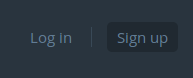
\includegraphics[width=0.3\textwidth]{apendice_manual_usuario/general_botones.png}
  \caption{Botones principales para el usuario anónimo}
  \label{fig:botones-1}
\end{figure}

Si es la primera vez que accede al sitio web deberá registrarse. Para ello, debe
pulsar en el botón \textbf{Sign up}, que se ve en la figura \ref{fig:botones-1}.

Tras ello, aparecerá el formulario de registro de usuario, que se ve en la
figura \ref{fig:registro}

\begin{figure}[hbtp]
  \centering
  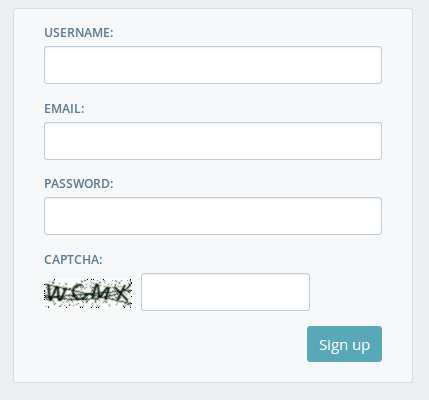
\includegraphics[width=0.5\textwidth]{apendice_manual_usuario/formulario_registro.png}
  \caption{Formulario de registro de usuario}
  \label{fig:registro}
\end{figure}

En el formulario deberá introducir los siguientes datos:

\begin{itemize}
\item \textbf{Nombre de usuario}. Debe tener 30 caracteres como máximo, y solo
  pueden usarse letras, números y guiones.
\item \textbf{Dirección de correo electrónico}. Asegúrese de que es una
  dirección de correo correcta.
\item \textbf{Contraseña}.
\item \textbf{Captcha}, usado para evitar el registro automático de bots. Deberá
  introducir los caracteres que se ven en la imagen. Si no consigue ver bien los
  caracteres, actualice la página y aparecerá una nueva imagen.
\end{itemize}

Tras introducir los datos, deberá pulsar el botón \textbf{Sign up} del
formulario. Si el registro es correcto, el sistema dará de alta su usuario y
mostrará la pantalla \ref{fig:registro-correcto}. Si no, volverá a aparecer el
formulario con información sobre los errores en los datos.

\begin{figure}[hbtp]
  \centering
  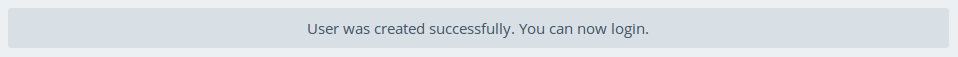
\includegraphics[width=\textwidth]{apendice_manual_usuario/pantalla_register_completo.png}
  \caption{Mensaje indicando el registro correcto}
  \label{fig:registro-correcto}
\end{figure}

\subsection{Inicio de sesión}

Una vez que haya registrado su usuario, deberá pulsar en el botón \textbf{Log
  in}, como aparece en la imagen \ref{fig:botones-1}. Esto le llevará al
formulario de inicio de sesión que aparece en la figura \ref{fig:login}

\begin{figure}[hbtp]
  \centering
  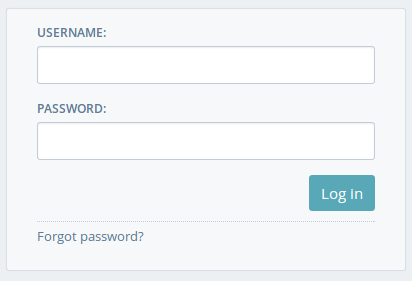
\includegraphics[width=0.5\textwidth]{apendice_manual_usuario/general_formulario_login.png}
  \caption{Formulario de inicio de sesión}
  \label{fig:login}
\end{figure}

Deberá introducir su nombre de usuario y la contraseña que escribió al
registrarse, y posteriormente pulsar en el botón \textbf{Log in} del
formulario. Si los datos son correctos, será llevado al panel principal de la
web, donde podrá gestionar sus chequeos. Si no son correctos, volverá a aparecer
el formulario, con información sobre los errores encontrados.

\subsection{Recuperación de contraseña}

Si se registró como usuario pero no recuerda su contraseña es posible
recuperarla.

Para ello, vaya al formulario de inicio de sesión como ser ha explicado en el
paso anterior. En ese formulario, en la zona inferior, verá un enlace titulado
\textbf{Forgot password?} que deberá pulsar. Después de hacerlo se mostrará el
formulario de recuperación de contraseña, ilustrado en la figura
\ref{fig:formulario-reset}.

\begin{figure}[hbtp]
  \centering
  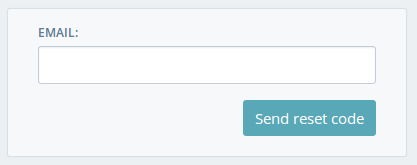
\includegraphics[width=0.5\textwidth]{apendice_manual_usuario/general_formulario_reset.png}
  \caption{Formulario de recuperación de contraseña}
  \label{fig:formulario-reset}
\end{figure}

En este formulario deberá introducir la dirección de correo electrónico que
utilizó al registrarse, y pulsar el botón \textbf{Send reset code}. Si lo hace
correctamente, aparecerá la pantalla de confirmación que se ve en la figura
\ref{fig:pantalla-reset-enviado}.

\begin{figure}[hbtp]
  \centering
  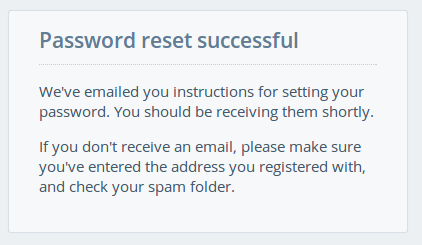
\includegraphics[width=0.5\textwidth]{apendice_manual_usuario/pantalla_reset_enviado.png}
  \caption{Pantalla de confirmación de envío de código de reinicio}
  \label{fig:pantalla-reset-enviado}
\end{figure}

El sistema habrá enviado un enlace a su dirección de correo electrónico. Deberá
pulsar el enlace que aparece en ese correo. Asegúrese de que recibe
correctamente el correo. Si no lo recibe, revise la carpeta de correo no
deseado. El enlace del correo le llevará a un formulario de reseteo de
contraseña como el que aparece en la figura \ref{fig:formulario-reset-2}.

\begin{figure}[hbtp]
  \centering
  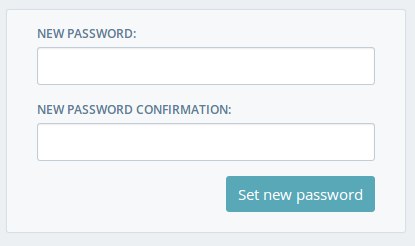
\includegraphics[width=0.5\textwidth]{apendice_manual_usuario/general_formulario_reset_2.png}
  \caption{Pantalla para la introducción de la nueva contraseña}
  \label{fig:formulario-reset-2}
\end{figure}

En este formulario deberá escribir la nueva contraseña de su cuenta dos veces,
para confirmar que la escribe correctamente. Tras ello, deberá pulsar el botón
\textbf{Set new password}, lo cual confirmará los cambios. 

Tras este proceso, podrá iniciar sesión como se ha descrito previamente, esta
vez utilizando la nueva contraseña.


\subsection{Pantalla de listado de chequeos}

\begin{figure}[hbtp]
  \centering
  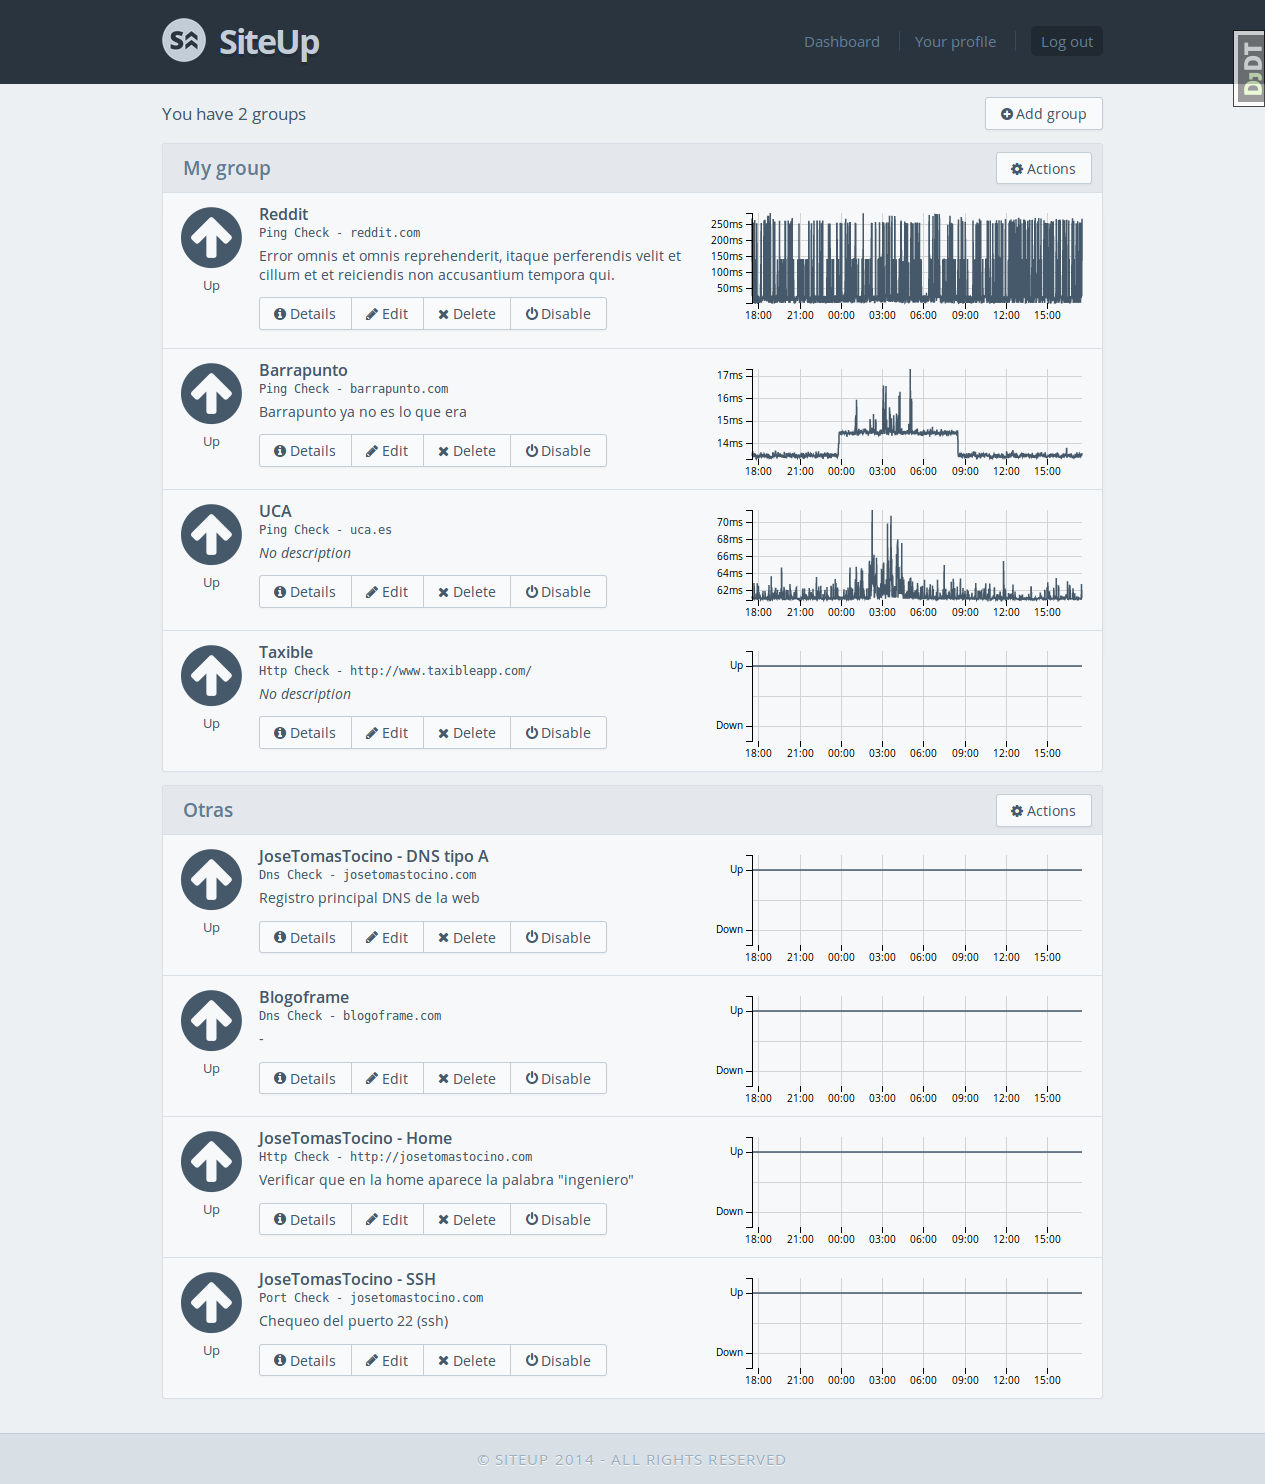
\includegraphics[width=0.8\textwidth]{apendice_manual_usuario/pantalla-dashboard.png}
  \caption{Panel de control}
  \label{fig:dashboard}
\end{figure}

\begin{figure}[hbtp]
  \centering
  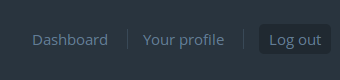
\includegraphics[width=0.4\textwidth]{apendice_manual_usuario/general_botones_2.png}
  \caption{Botones principales para el usuario logueado}
  \label{fig:botones-2}
\end{figure}

En la figura \ref{fig:dashboard} se puede ver el aspecto del panel de control de
la plataforma web SiteUp. Desde este panel podrá hacer una gran cantidad de
acciones, desde crear grupos de chequeos hasta editar sus detalles de usuario.

Es posible acceder a esta pantalla desde cualquier sitio de la web si está
logueado, pulsando en el botón \textbf{Dashboard} de la cabecera de la web, tal
y como se ve en la figura \ref{fig:botones-2}.

\subsection{Cerrar sesión}

Si ha iniciado sesión y desea cerrarla, debe dirigirse a los botones
principales, situados en el lado derecho de la cabecera de la web, tal y como
aparecen en la figura \ref{fig:botones-2}. Deberá pulsar el botón \textbf{Log
  out}, tras lo cual se cerrara su sesión y será redirigido a la pantalla
inicial de SiteUp.

\subsection{Edición de datos de usuario}

Si desea editar alguno de los datos de usuario que ingresó cuando hizo el
registro, deberá primero pulsar el botón \textbf{Your profile}, situado en la
cabecera de la web. Es el segundo de los botones que aparecen, tal y como se ve
en la figura \ref{fig:botones-2}.

Una vez hecho esto, aparecerá el formulario de edición de usuario, ilustrado en
la figura \ref{fig:formulario-usuario}, en el que verá sus actuales datos de
usuario. 

\begin{figure}[hbtp]
  \centering
  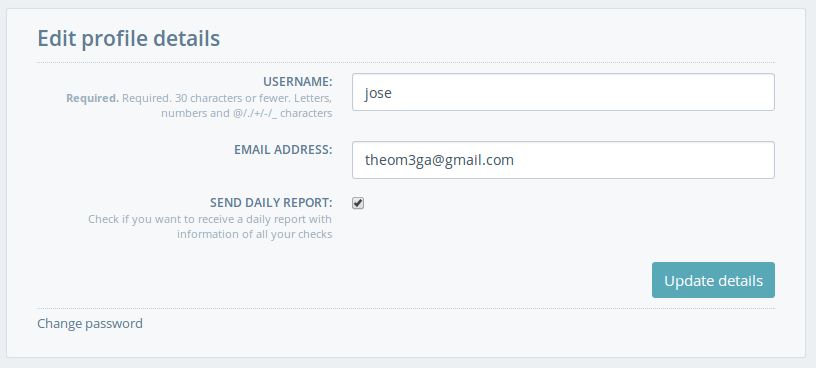
\includegraphics[width=0.8\textwidth]{apendice_manual_usuario/pantalla_perfil_usuario.png}
  \caption{Pantalla de edición del perfil de usuario}
  \label{fig:formulario-usuario}
\end{figure}

En este formulario podrá editar:

\begin{itemize}
\item Su \textbf{nombre} de usuario.
\item Su \textbf{dirección} de correo electrónico.
\item Si desea o no recibir \textbf{resúmenes diarios} sobre el estado de sus chequeos.
\end{itemize}

Una vez editados los datos que desee deberá pulsar el botón \textbf{Update
  details}. También podrá editar su contraseña pulsando el botón \textbf{Change
  password}, situado al pie del formulario a la izquierda.


\subsection{Creación de grupo de chequeos}

En SiteUp, los chequeos se organizan en \textbf{grupos de chequeos}, lo que
permite trabajar con ellos más fácilmente a la hora de activarlos, desactivarlos
o borrarlos. 

Para crear un grupo de chequeos deberá pulsar el botón \textbf{Add group},
situado en la zona superior derecha del panel principal. El botón puede verse en
la figura \ref{fig:crear-grupo}.

\begin{figure}[hbtp]
  \centering
  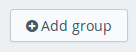
\includegraphics[width=0.3\textwidth]{apendice_manual_usuario/grupo_boton_nuevo.png}
  \caption{Botón para crear nuevo grupo de chequeos}
  \label{fig:crear-grupo}
\end{figure}

Tras pulsar el botón aparecerá el formulario de creación de nuevo grupo. En él
deberá introducir los datos del nuevo grupo. En particular:

\begin{itemize}
\item El \textbf{título} que identifica al grupo.
\end{itemize}

Tras ello, deberá pulsar el botón \textbf{Create group}, y el grupo será creado

\begin{figure}[H]
  \centering
  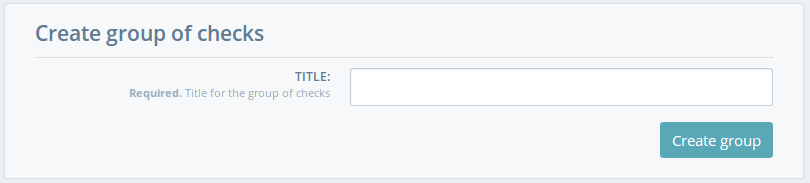
\includegraphics[width=0.8\textwidth]{apendice_manual_usuario/grupo_formulario_crear.png}
  \caption{Formulario de creación de grupo de chequeos}
  \label{fig:}
\end{figure}


\subsection{Operaciones con grupos de chequeos}

En la figura~\ref{fig:operaciones-grupo} se puede ver el menú de operaciones
disponibles para un grupo de chequeos. Este menú aparece en el panel principal,
al lado derecho junto al título de cada grupo de chequeos.

\begin{figure}[hbtp]
  \centering
  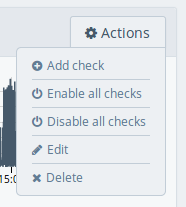
\includegraphics[width=0.5\textwidth]{apendice_manual_usuario/grupo_submenu_acciones.png}
  \caption{Menú de acciones de grupo}
  \label{fig:operaciones-grupo}
\end{figure}

\subsubsection{Edición de grupo de chequeos}

En el menú de operaciones del grupo de chequeos, pulse el botón
\textbf{Edit}. Aparecerá un formulario similar al de creación de grupo, en el
que podrá editar el título del grupo de chequeos.

\subsubsection{Borrado de grupo de chequeos}

Para borrar un grupo de chequeos, pulse el botón \textbf{Delete} en el menú de
operaciones del grupo. Aparecerá un formulario como el de la figura
\ref{fig:formulario-borrado-grupo}, pidiéndole confirmación del borrado. 

\begin{figure}[hbtp]
  \centering
  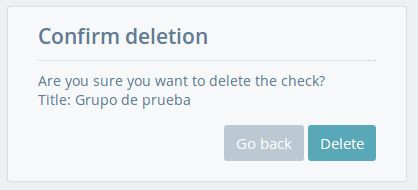
\includegraphics[width=0.5\textwidth]{apendice_manual_usuario/formulario_borrado_grupo}
  \caption{Formulario de confirmación de borrado}
  \label{fig:formulario-borrado-grupo}
\end{figure}

Si pulsa en el botón \textbf{Go back}, volverá al panel principal, cancelando el
borrado. Si pulsa el botón \textbf{Delete}, confirmará la operación y el sistema
borrará el grupo de chequeos, así como todos los chequeos que contenga.

\subsubsection{Activación y desactivación de grupo de chequeos}

Es posible activar y desactivar de forma grupal todos los chequeos de un
grupo. Para ello, deberá dirigirse al menú de operaciones del grupo y pulsar en
\textbf{Enable all checks} o en \textbf{Disable all checks}, según sea su decisión.

\subsection{Creación de chequeo}

\begin{figure}[hbtp]
  \centering
  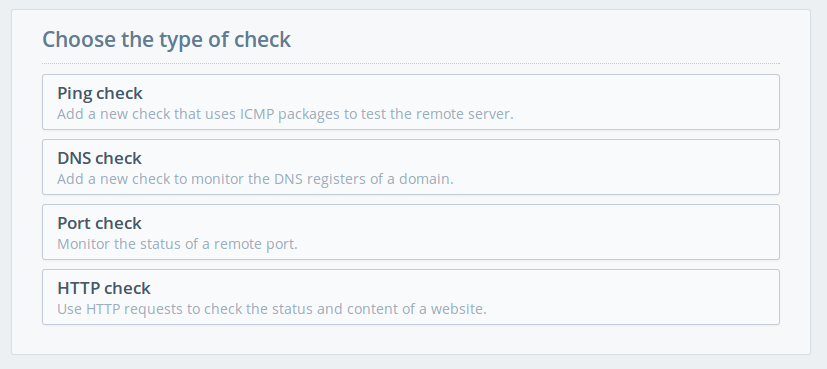
\includegraphics[width=0.8\textwidth]{apendice_manual_usuario/pantalla_seleccion_tipo.png}
  \caption{Pantalla de selección del tipo de chequeo a crear}
  \label{fig:seleccionar-tipo-check}
\end{figure}

Como se ha comentado previamente, el elemento principal de SiteUp es el
\textbf{chequeo}. El usuario da de alta chequeos dentro de un grupo, y estos
chequeos se lanzan periódicamente, generando datos.

Para crear un chequeo dentro de un grupo deberá ir al menú de operaciones del
grupo, que aparece en la figura \ref{fig:operaciones-grupo} y se sitúa a la
derecha del título de un grupo de chequeos. Dentro del menú, deberá pulsar la
opción \textbf{Add check}.



Tras esto aparecerá una pantalla en la que deberá seleccionar el tipo de chequeo
que desea crear. La pantalla es similar a la de la figura
\ref{fig:seleccionar-tipo-check}. Como se explicó en la introducción de este
manual, es posible crear cuatro tipo de chequeos: chequeos de ping, chequeos de
puerto, chequeos de registros DNS y chequeos por HTTP.

Si pulsa en el botón del tipo que desea crear, aparecerá un formulario con
campos para rellenar.

\subsubsection{Creación de un chequeo por ping}

\begin{figure}[hbtp]
  \centering
  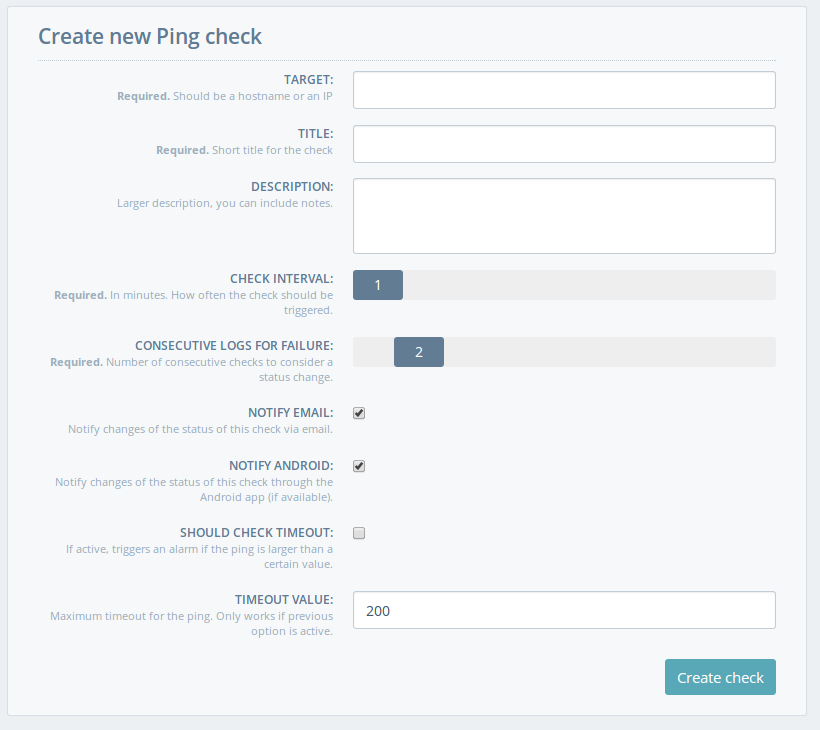
\includegraphics[width=0.8\textwidth]{apendice_manual_usuario/pantalla_crear_ping.png}
  \caption{Formulario de creación de chequeo por ping}
  \label{fig:crear-ping}
\end{figure}

El formulario para crear un chequeo de tipo ping aparece en la
figura~\ref{fig:crear-ping}. Los campos que deberá rellenar son los siguientes:

\begin{itemize}
\item \textbf{Target}: es el objetivo a chequear. Debe ser un \textit{hostname} o una IP.
\item \textbf{Título} del chequeo.
\item \textbf{Descripción} opcional del chequeo.
\item \textbf{Check interval}: intervalo entre chequeos, definido en minutos. El
  valor mínimo es de 1 minuto.
\item \textbf{Notify email}: indica si los cambios de estado en este chequeo
  deberán ser notificados por correo electrónico.
\item \textbf{Notify Android}: indica si los cambios de estado en este chequeo
  deberán ser notificados mediante la aplicación Android.
\item \textbf{Should check timeout}: indica si hay que verificar que el ping
  enviado vuelve dentro de un tiempo máximo determinado.
\item \textbf{Timeout value}: si la anterior opción está activa, este campo
  define el número de milisegundos que puede tardar en responder el servidor al
  ping, como máximo.
\end{itemize}

\subsubsection{Creación de un chequeo de puerto}

\begin{figure}[hbtp]
  \centering
  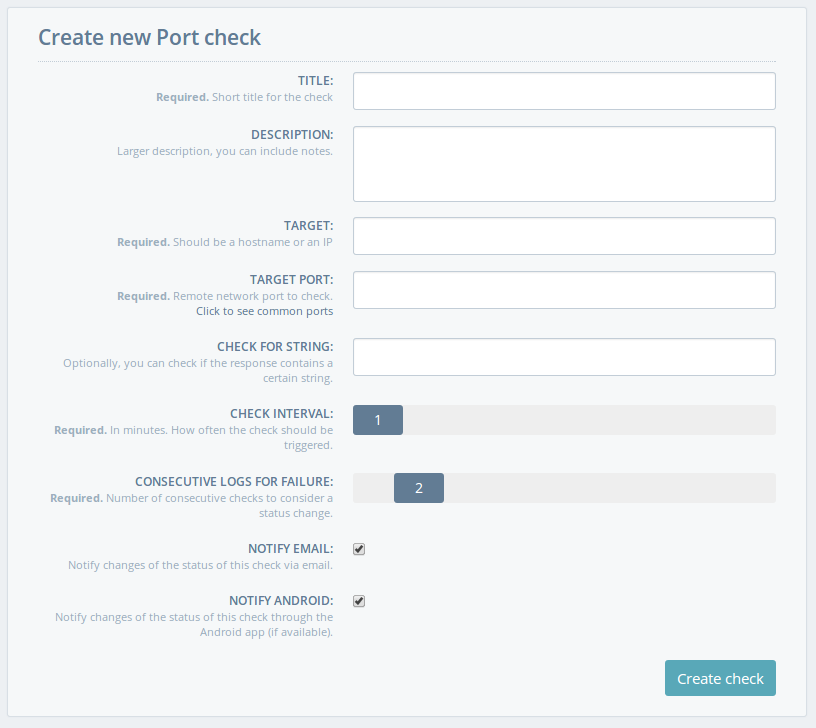
\includegraphics[width=0.8\textwidth]{apendice_manual_usuario/pantalla_crear_port.png}
  \caption{Formulario de creación de chequeo de puerto}
  \label{fig:crear-port}
\end{figure}

El formulario para crear un chequeo de puertos aparece en la
figura~\ref{fig:crear-port}. Los campos que deberá rellenar son los siguientes:

\begin{itemize}
\item \textbf{Título} del chequeo.
\item \textbf{Descripción} opcional del chequeo.
\item \textbf{Target}: es el objetivo a chequear. Debe ser un \textit{hostname} o una IP.
\item \textbf{Target port}: es el puerto a chequear. Debe ser un entero.
\item \textbf{Check for string}: opcionalmente, se puede indicar una cadena que
  debe estar presente en la respuesta al conectar con el puerto.
\item \textbf{Check interval}: intervalo entre chequeos, definido en minutos. El
  valor mínimo es de 1 minuto.
\item \textbf{Notify email}: indica si los cambios de estado en este chequeo
  deberán ser notificados por correo electrónico.
\item \textbf{Notify Android}: indica si los cambios de estado en este chequeo
  deberán ser notificados mediante la aplicación Android.
\end{itemize}

\subsubsection{Creación de un chequeo de DNS}

\begin{figure}[hbtp]
  \centering
  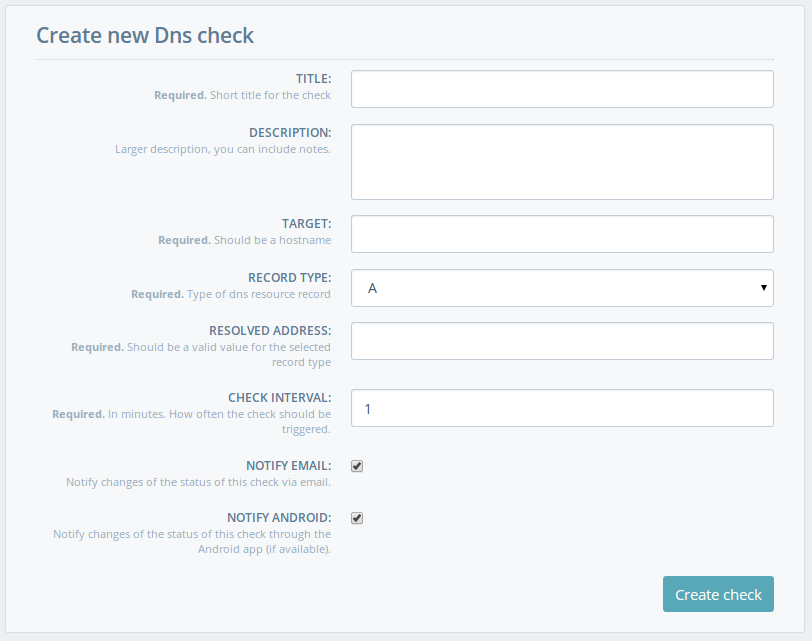
\includegraphics[width=0.8\textwidth]{apendice_manual_usuario/pantalla_crear_dns.png}
  \caption{Formulario de creación de chequeo de registro DNS}
  \label{fig:crear-dns}
\end{figure}

El formulario para crear un chequeo de registro DNS aparece en la figura
\ref{fig:crear-dns}. Los campos que deberá rellenar son los siguientes:

\begin{itemize}
\item \textbf{Título} del chequeo.
\item \textbf{Descripción} opcional del chequeo.
\item \textbf{Target}: es el objetivo a chequear. Debe ser un \textit{hostname}.
\item \textbf{Record type}: indica el tipo de registro a chequear. Puede ser A, AAAA, CNAME, TXT y MX.
\item \textbf{Resolved address}: indica el contenido que debe tener el registro.
\item \textbf{Check interval}: intervalo entre chequeos, definido en minutos. El
  valor mínimo es de 1 minuto.
\item \textbf{Notify email}: indica si los cambios de estado en este chequeo
  deberán ser notificados por correo electrónico.
\item \textbf{Notify Android}: indica si los cambios de estado en este chequeo
  deberán ser notificados mediante la aplicación Android.
\end{itemize}

\subsubsection{Creación de un chequeo por HTTP}

\begin{figure}[hbtp]
  \centering
  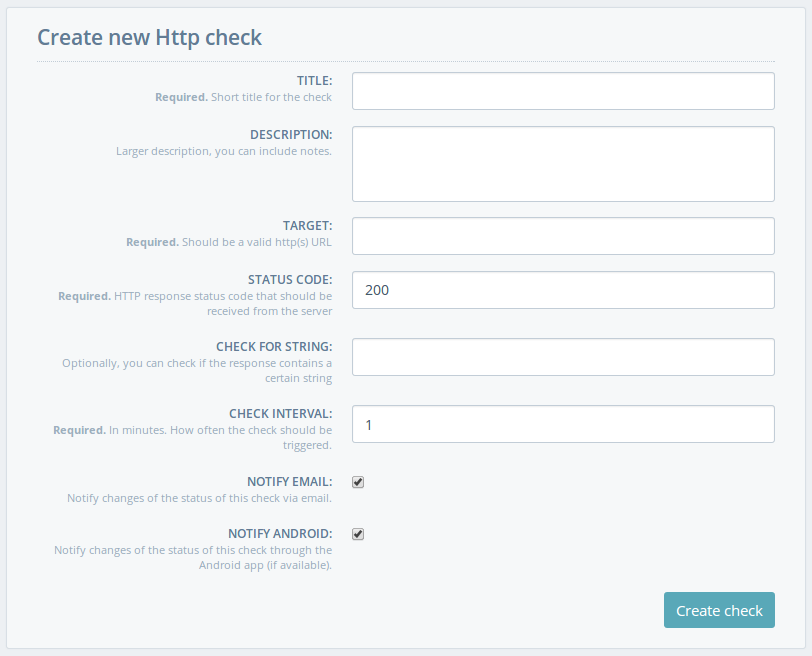
\includegraphics[width=0.8\textwidth]{apendice_manual_usuario/pantalla_crear_http.png}
  \caption{Formulario de creación de chequeo por HTTP}
  \label{fig:crear-http}
\end{figure}

El formulario para crear un chequeo por HTTP aparece en la figura
\ref{fig:crear-http}. Los campos que deberá rellenar son los siguientes:

\begin{itemize}
\item \textbf{Título} del chequeo.
\item \textbf{Descripción} opcional del chequeo.
\item \textbf{Target}: es el objetivo a chequear. Debe ser una URL.
\item \textbf{Status code}: es el código de estado que deberá devolver la petición.
\item \textbf{Check for string}: opcionalmente, se puede indicar una cadena que
  debe estar presente en la respuesta a la petición.
\item \textbf{Check interval}: intervalo entre chequeos, definido en minutos. El
  valor mínimo es de 1 minuto.
\item \textbf{Notify email}: indica si los cambios de estado en este chequeo
  deberán ser notificados por correo electrónico.
\item \textbf{Notify Android}: indica si los cambios de estado en este chequeo
  deberán ser notificados mediante la aplicación Android.
\end{itemize}


\subsection{Operaciones con chequeos}

\begin{figure}[hbtp]
  \centering
  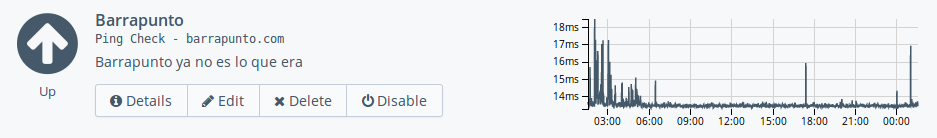
\includegraphics[width=\textwidth]{apendice_manual_usuario/chequeo_valido.png}
  \caption{Aspecto de un chequeo válido}
  \label{fig:chequeo}
\end{figure}

Una vez creado un chequeo, aparecerá en el panel de control con el aspecto de la
figura~\ref{fig:chequeo}. Como se aprecia en la figura, se muestra mediante un
icono el estado del chequeo, los datos (título, tipo, descripción) y una gráfica
que ilustra el estado del chequeo en las últimas 24 horas.

\begin{figure}[hbtp]
  \centering
  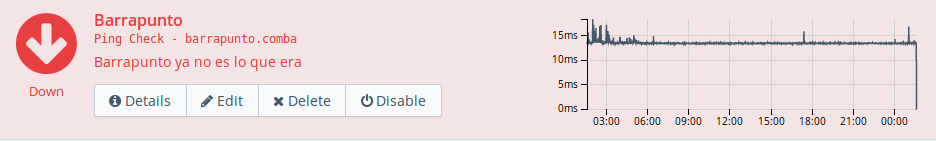
\includegraphics[width=\textwidth]{apendice_manual_usuario/chequeo_invalido.png}
  \caption{Aspecto de un chequeo en estado de error}
  \label{fig:chequeo-invalido}
\end{figure}

Si un chequeo detecta un error, cambia de apariencia, pasando a tener el aspecto
que ofrece la figura \ref{fig:chequeo-invalido}. Además, según se haya
configurado en las opciones del chequeo, se envía una notificación al usuario
informando del cambio de estado del chequeo.

Cuando se ve en la lista general de chequeos, cada chequeo tiene una serie de
botones que permiten llevar a cabo operaciones diversas, que se detallan a
continuación.

\subsubsection{Activación y desactivación de un chequeo}

Para desactivar un chequeo, tiene que pulsar el botón \textbf{Disable} de la
botonera, que solo aparecerá si el chequeo está activado. De igual modo, si el
chequeo está desactivado, el botón que aparecerá tendrá la etiqueta
\textbf{Enable}, que podrá pulsar para activarlo.

\subsubsection{Borrado de un chequeo}

En la botonera se sitúa el botón \textbf{Delete}, que podrá pulsar para borrar
el chequeo. Aparecerá un formulario pidiéndole confirmación. Si confirma la
acción, se procederá al borrado del chequeo y todos los datos dependientes de
éste.

\subsubsection{Edición de un chequeo}

Si desea editar un chequeo debe pulsar el botón \textbf{Edit}, situado en la
botonera del chequeo. Aparecerá un formulario similar al de creación de chequeo,
pero con los datos actuales ya introducidos. Puede modificar los datos que desee
y confirmar los cambios pulsando el botón \textbf{Update check} del formulario.

\subsubsection{Vista de detalle del chequeo}

\begin{figure}[hbtp]
  \centering
  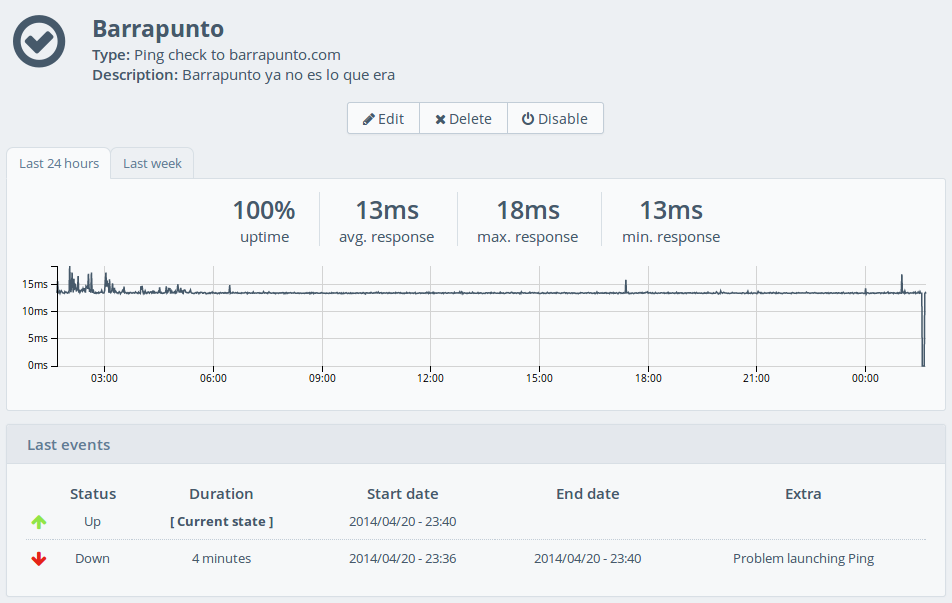
\includegraphics[width=\textwidth]{apendice_manual_usuario/pantalla_detalle_chequeo.png}
  \caption{Pantalla de detalle de chequeo}
  \label{fig:detalle-chequeo}
\end{figure}

En la botonera del chequeo, en el panel de control, verá un botón
\textbf{Details}. Si lo pulsa será llevado a la pantalla de vista de detalle del
chequeo, que se ilustra en la figura \ref{fig:detalle-chequeo}. Esta pantalla
ofrece mucha información sobre el chequeo. En particular:

\begin{itemize}
\item En la parte superior se sitúa la información general:
  \begin{itemize}
  \item Icono con el estado del chequeo.
  \item Título.
  \item Tipo de chequeo.
  \item Descripción.
  \item Botonera de acciones.
  \end{itemize}

\item En la parte media de la pantalla se sitúa un bloque con pestañas. Mediante
  estas pestañas es posible indicar sobre qué periodo de tiempo queremos
  visualizar los datos: últimas 24 horas, última semana, último mes, etc. La
  información disponible es la siguiente:

  \begin{itemize}
  \item Porcentaje de \textit{uptime} del chequeo.
  \item \textit{(Solo chequeos tipo ping)} Tiempo de respuesta mínimo, máximo y promedio.
  \item Gráfica con el estado del chequeo.
  \item Eventos durante ese periodo de tiempo. Un evento es un cambio de estado
    del chequeo, con la siguiente información:
    \begin{itemize}
    \item Tipo de cambio de estado (\textit{Up}, \textit{Down}).
    \item Duración del estado.
    \item Hora de comienzo del estado.
    \item Hora de fin del estado. Si es el estado en el que el chequeo se
      encuentra actualmente, no aparecerá ninguna fecha.
    \item Extra: muestra información adicional para estados de error.
    \end{itemize}
  \end{itemize}

\end{itemize}

\subsection{Recepción de notificaciones por correo electrónico}

\subsubsection{Notificaciones de cambio de estado}

Cuando el sistema detecte un cambio de estado en un chequeo, y esté activada la
notificación por correo electrónico, se enviará un email como el que aparece en
la figura \ref{fig:email-estado}.

\begin{figure}[hbtp]
  \centering
  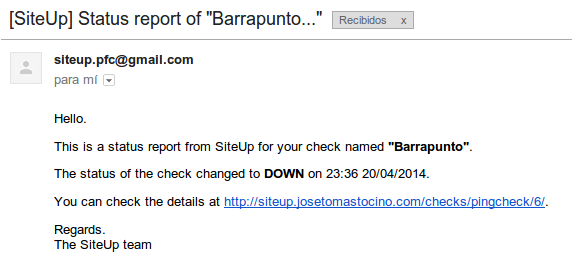
\includegraphics[width=0.7\textwidth]{apendice_manual_usuario/email_estado.png}
  \caption{Email de notificación de cambio de estado}
  \label{fig:email-estado}
\end{figure}

En ese email se le indicará el título del chequeo, el nuevo estado, la fecha y
hora en la que ha pasado al nuevo estado, y un enlace directo al panel de
detalle del chequeo en SiteUp, de forma que pueda obtener más información.

\subsubsection{Notificaciones de resumen diarias}

Si ha activado el envío de resúmenes diarios sobre el estado de sus chequeos, el
sistema enviará todos los días un correo electrónico con información. El aspecto
del correo que recibirá se puede ver en la figura \ref{fig:email-resumen}

\begin{figure}[hbtp]
  \centering
  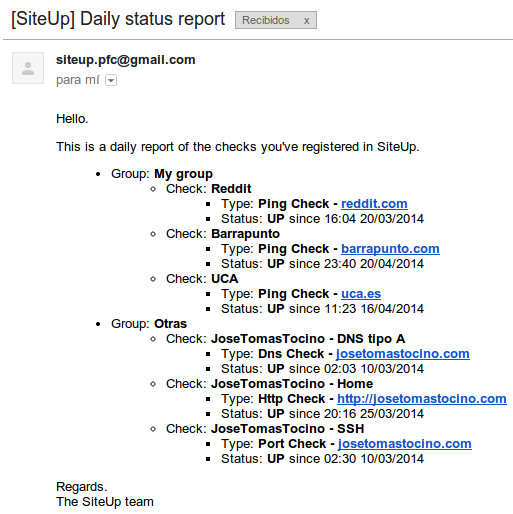
\includegraphics[width=0.7\textwidth]{apendice_manual_usuario/email_resumen.png}
  \caption{Email diario de resumen}
  \label{fig:email-resumen}
\end{figure}


\section{Uso de la aplicación móvil}

La aplicación móvil \textbf{SiteUp Client} es una aplicación para para el
sistema operativo Android que permite a sus usuarios revisar los chequeos que
tiene dados de alta en la plataforma web SiteUp, así como recibir de manera
instantánea notificaciones \textit{push} sobre el estado de sus chequeos.

\subsection{Instalación}

La aplicación móvil se instala copiando y ejecutando el fichero APK en el
dispositivo. En un futuro se podrá encontrar en la \textit{Play Store} de
Google.

\subsection{Lanzamiento}

En la figura~\ref{fig:manual-android-launcher} se puede observar el aspecto de
la aplicación \textbf{SiteUp Client} en el lanzador de Android. Para ejecutarla,
simplemente pulse sobre el icono de la aplicación.

\begin{figure}[htbp]
  \centering
  
\includegraphics[width=0.4\textwidth]{5_diseno/android-1}
  \caption{Icono de SiteUp en el lanzador}
  \label{fig:manual-android-launcher}
\end{figure}

\subsection{Carga de la aplicación}

Tras lanzar la aplicación, el sistema cargará los datos necesarios y se
comunicará con los servidores de Google para obtener los datos necesarios. La
apariencia de la aplicación durante este proceso se puede ver en la figura
\ref{fig:manual-android-login}.

\begin{figure}[htbp]
  \centering
  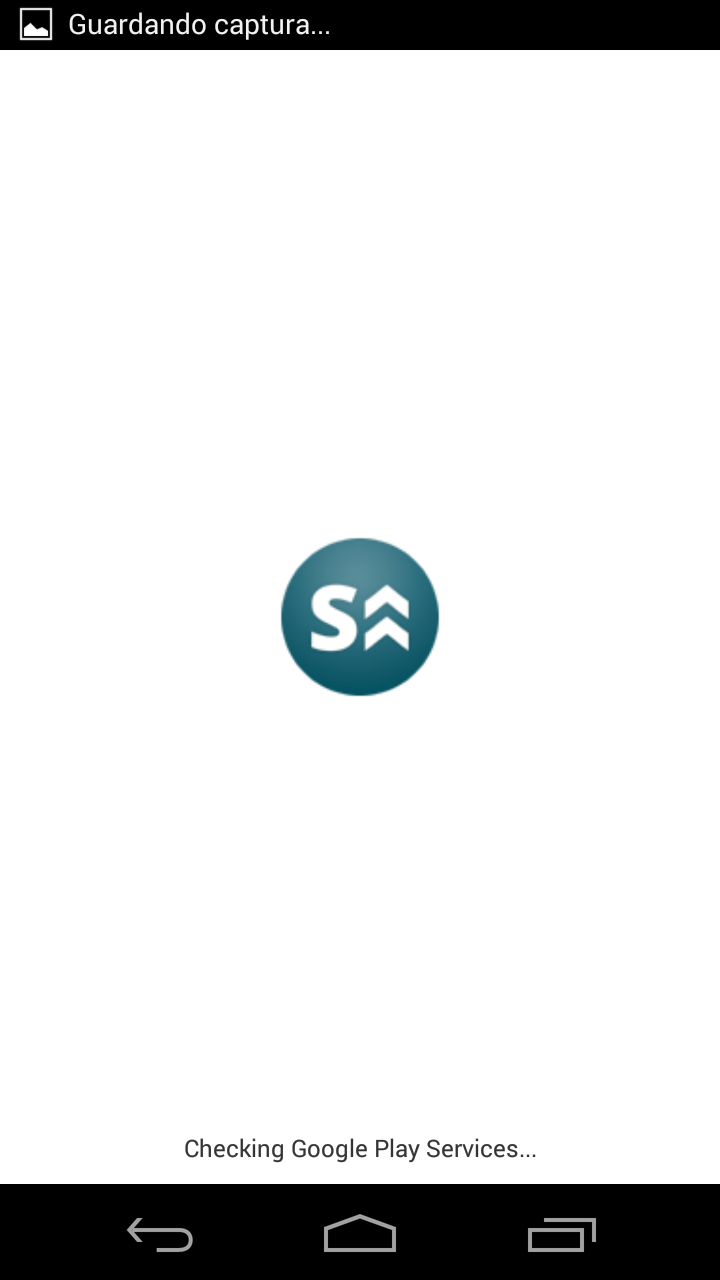
\includegraphics[width=0.4\textwidth]{5_diseno/android-2}
  \caption{Pantalla de carga de la aplicación móvil}
  \label{fig:manual-android-loading}
\end{figure}

\subsection{Inicio de sesión}

Tras la carga, la primera vez que lance la aplicación será necesario que inicie
sesión con las credenciales que utilizó en la plataforma web. Para ello, tendrá
que introducir su nombre de usuario y contraseña en el formulario que aparece en
la figura~\ref{fig:manual-android-loading}, y pulsar el botón \textbf{Sign in}.

\begin{figure}[htbp]
  \centering
  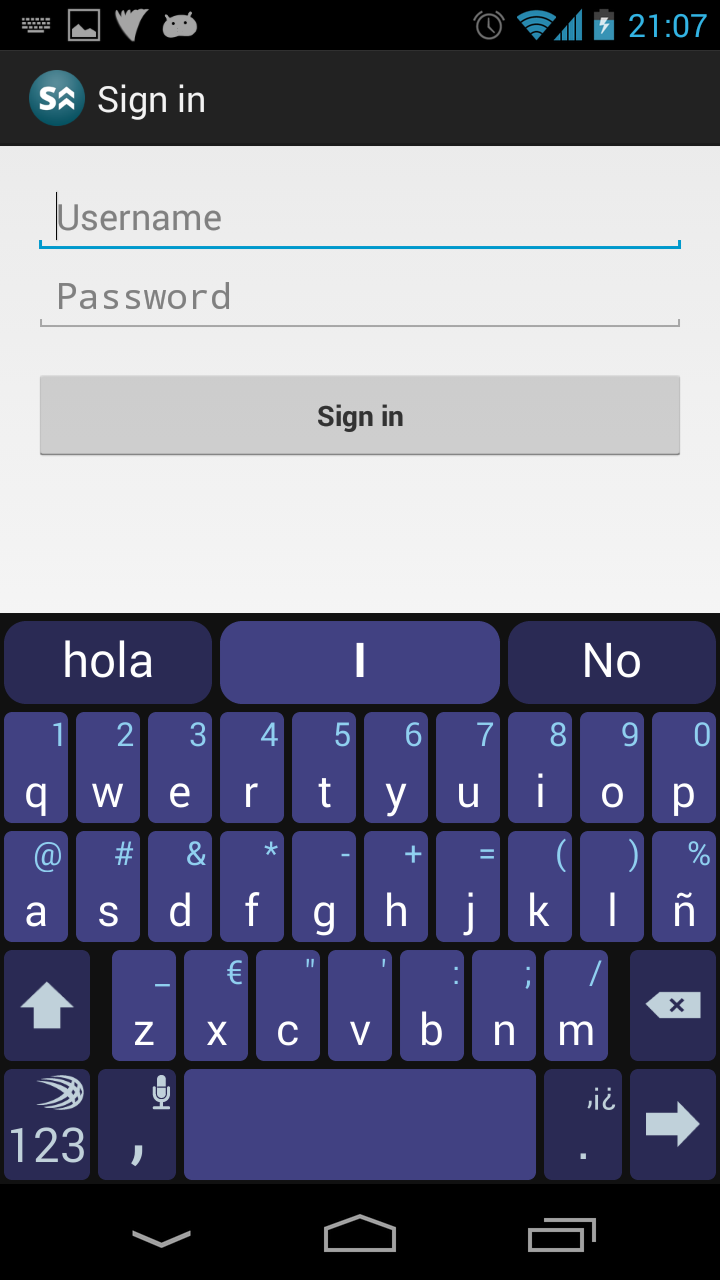
\includegraphics[width=0.4\textwidth]{5_diseno/android-3}
  \caption{Pantalla de inicio de sesión de la aplicación móvil}
  \label{fig:manual-android-login}
\end{figure}

La aplicación móvil se comunicará con los servidores centrales de SiteUp,
validará sus credenciales de usuario y, si son correctas, le dará acceso al
sistema. Si las credenciales de usuario no son correctas, el formulario mostrará
un error.

\subsection{Revisión de chequeos}

Si ha iniciado sesión correctamente, tendrá la opción de revisar la lista de
chequeos que tiene dados de alta en la plataforma web \textbf{SiteUp}. La
apariencia de la lista de chequeos es igual a la de la
figura~\ref{fig:manual-android-dashboard}.

\begin{figure}[hbtp]
  \centering
  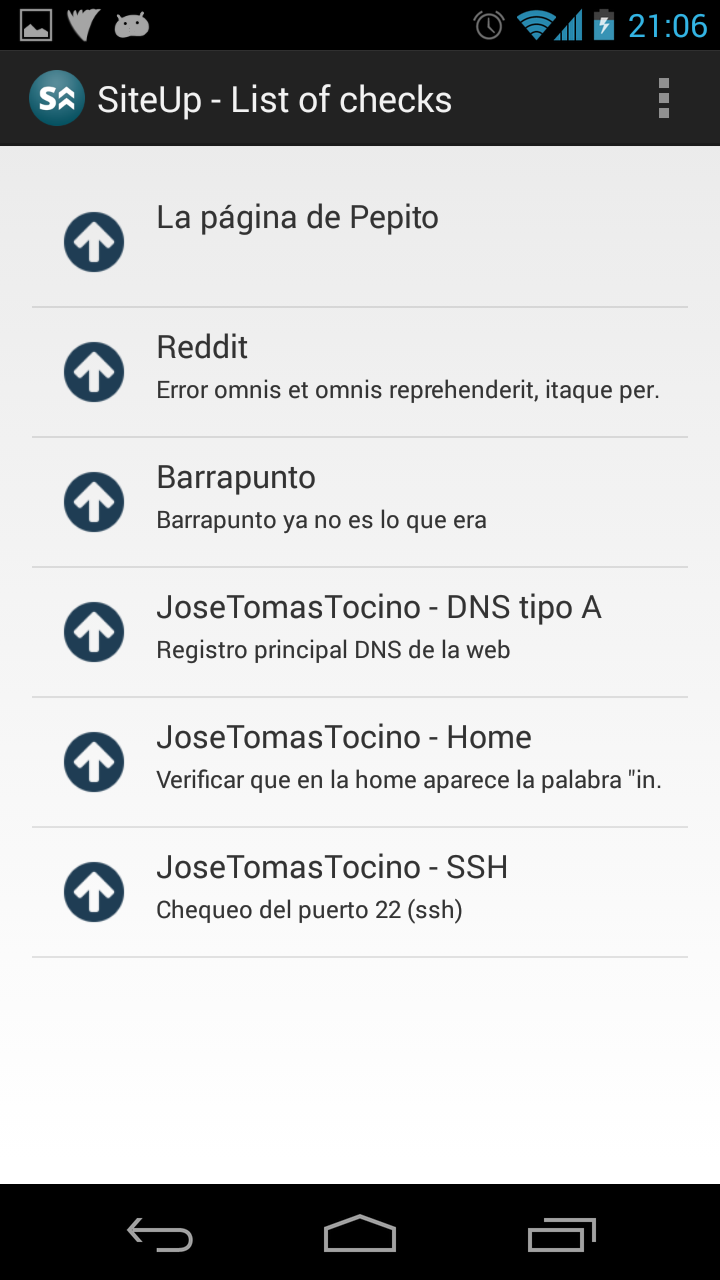
\includegraphics[width=0.4\textwidth]{5_diseno/android-4}
  \caption{Pantalla de chequeos de la aplicación móvil}
  \label{fig:manual-android-dashboard}
\end{figure}

Si pulsa en cualquiera de los chequeos, será redirigido a la plataforma web, que
podrá navegar sin problema gracias a que se encuentra preparada para su uso en
dispositivos móviles.

\subsection{Recepción de notificaciones}

La utilidad principal de la aplicación es la posibilidad de recibir
notificaciones en cualquier momento provenientes del servidor -- conocidas como
notificaciones \textit{push}. 

El procedimiento es transparente al usuario. Simplemente lance la aplicación e
inice sesión. Tras hacer esto, la aplicación estará preparada para recibir
notificaciones desde el servidor.

Cuando se reciba una notificación, la aplicación mostará un mensaje en el área
de notificaciones del móvil, con información resumida. Puede ver el aspecto de
la notificación en la figura \ref{fig:manual-android-notification}. Si pulsa en
la notificación será llevado a los detalles del chequeo para obtener más
detalles sobre el origen del aviso.

\begin{figure}[hbtp]
  \centering
  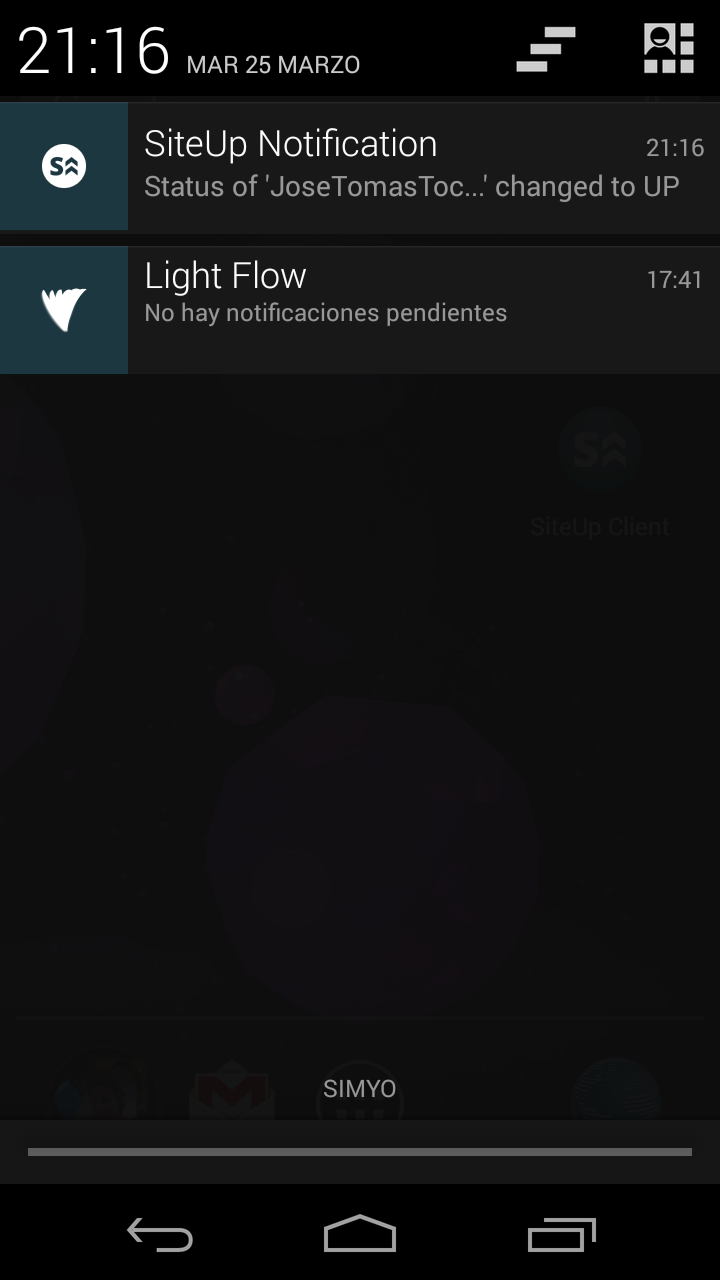
\includegraphics[width=0.4\textwidth]{5_diseno/android-5}
  \caption{Aspecto de las notificaciones}
  \label{fig:manual-android-notification}
\end{figure}



%%% Local Variables:
%%% mode: latex
%%% TeX-master: "../memoria"
%%% End:
